\section{The Hopf bundles}\label{ch:hopf}

This section proves Theorem~\ref{thm:A}. The four cases are treated at once; the only place where the octonions need care is Lemma~\ref{lem:artin}.

\subsection{The normed division algebras}\label{sec:algebras}

The algebras $\R\subset\C\subset\Hq\subset\Oc$ are obtained by the Cayley--Dickson construction. If $A$ is a real algebra with unit and an involution $x\mapsto\bar x$, then $A\oplus A$ with
\begin{equation}\label{eq:cd}
(a,b)(c,d)=\bigl(ac-\bar d b,\;da+b\bar c\bigr),\qquad \overline{(a,b)}=(\bar a,-b),
\end{equation}
is again a real algebra with unit $(1,0)$ and involution. Starting from $\R$ with the trivial involution one obtains $\C$, $\Hq$ and $\Oc$, of dimensions $2,4,8$.\footnote{Doubling $\Oc$ once more gives the sedenions, which have zero divisors; this is one way to see that the list stops. The theorem that it stops is Hurwitz's: a finite-dimensional real algebra with unit and a multiplicative positive definite norm is one of $\R,\C,\Hq,\Oc$ \cite[Section~2]{Bae02}. We do not need it, since Adams' theorem (I4) gives the stronger topological statement.} We collect the facts that are used, with references.

\begin{enumerate}[label=(D\arabic*)]
\item\label{D:norm} $x\bar x=\bar x x=|x|^2$ is the Euclidean norm squared, and $|xy|=|x|\,|y|$ for all $x,y\in\K$ \cite[Section~2.2]{Bae02}.
\item\label{D:conj} $\overline{xy}=\bar y\,\bar x$, and $\bar x=2\Re x-x$, where $\Re x=\tfrac12(x+\bar x)\in\R$ is the real part \cite[Section~2.2]{Bae02}.
\item\label{D:inner} The Euclidean inner product is $\langle x,y\rangle=\Re(x\bar y)=\Re(\bar x y)$, and $\langle xa,b\rangle=\langle a,\bar x b\rangle$, $\langle ax,b\rangle=\langle a,b\bar x\rangle$ \cite[Chapter~III]{Sch66}.
\item\label{D:artin} (Artin) Any two elements of $\K$ generate an associative subalgebra (input (I3); \cite[Theorem~3.1]{Sch66}).
\end{enumerate}
For $\K=\R,\C,\Hq$ all four are immediate, since these algebras are associative. The identities \ref{D:norm}--\ref{D:inner} are checked by direct computation from \eqref{eq:cd} for $\Oc$, and they are verified numerically, together with Artin's theorem and the Moufang identities, by the programs of Appendix~\ref{app:checks}.

\begin{lemma}\label{lem:artin}
Let $x,y\in\K$ with $y\neq0$, and put $y^{-1}=\bar y/|y|^2$. Then
\[
(xy)y^{-1}=x,\qquad (xy^{-1})y=x,\qquad y^{-1}(yx)=x,\qquad (xy)\bar y=|y|^2x,\qquad x(\bar x y)=|x|^2y .
\]
\end{lemma}

\begin{proof}
By \ref{D:conj}, $\bar y=2\Re y-y$ lies in the subalgebra generated by $1$ and $y$, so $x$, $y$, $\bar y$, $y^{-1}$ and $\bar x$ all lie in the subalgebra $A$ generated by $x$ and $y$. By Artin's theorem $A$ is associative, so $(xy)y^{-1}=x(yy^{-1})=x$, and similarly for the other identities, using $y\bar y=|y|^2$ and $\bar x x=|x|^2$ from \ref{D:norm}.
\end{proof}

For $x\in\K$ let $\ell_x\colon\K\to\K$, $\ell_x(c)=xc$, be left multiplication. It is $\R$-linear, and by \ref{D:norm} it multiplies lengths by $|x|$. Hence for $x\neq0$ it is a similarity of ratio $|x|$, with inverse $\ell_{x^{-1}}$ by Lemma~\ref{lem:artin}, and for $|x|=1$ it is orthogonal. We obtain a smooth map
\begin{equation}\label{eq:clutch}
\tau\colon S^{d-1}\to \mathrm{O}(d),\qquad \tau(x)=\ell_x .
\end{equation}

\begin{remark}\label{rem:notgroup}
For $\K=\R,\C,\Hq$ the unit sphere $S^{d-1}$ is a group and $\tau$ is a homomorphism, $\ell_x\ell_y=\ell_{xy}$. For $\Oc$ this fails: $\ell_x\ell_y=\ell_{xy}$ for all $x,y$ would make $\Oc$ associative. The unit sphere $S^7$ is not a group, and no Lie group structure on $S^7$ exists at all, since the only spheres that are Lie groups are $S^0$, $S^1$ and $S^3$.\footnote{A compact connected Lie group $G$ of positive dimension has $H^3(G;\R)\neq0$, since the bi-invariant $3$-form $(X,Y,Z)\mapsto\langle[X,Y],Z\rangle$ is closed and not exact when $G$ is not a torus; a torus that is a sphere is $S^1$. So a sphere $S^n$ that is a Lie group has $n=1$ or $n=3$.} The construction below uses only the maps $\ell_x$ and Lemma~\ref{lem:artin}, and it works uniformly.
\end{remark}

\subsection{The tautological bundle}\label{sec:taut}

For $x\in\K$ let $L_x=\{(xc,c):c\in\K\}$ and $L_\infty=\K\times\{0\}$, as in the Introduction. These are $d$-dimensional real subspaces of $\K^2$; $L_x$ is the graph of $\ell_x$ over the second factor.

\begin{proposition}\label{prop:lines}
Every nonzero vector $(a,b)\in\K^2$ lies in exactly one of the subspaces $L_x$, $x\in\K\cup\{\infty\}$: in $L_{ab^{-1}}$ if $b\neq0$, and in $L_\infty$ if $b=0$. Distinct subspaces meet only in $0$.
\end{proposition}

\begin{proof}
If $b=0$ then $(a,0)\in L_\infty$, and $(a,0)\notin L_x$ for $x\in\K$, since $(a,0)=(xc,c)$ forces $c=0$ and then $a=0$. If $b\neq0$, then $(a,b)\notin L_\infty$, and $(a,b)=(xc,c)$ holds exactly when $c=b$ and $a=xb$. The equation $xb=a$ has the solution $x=ab^{-1}$, because $(ab^{-1})b=a$ by Lemma~\ref{lem:artin}, and no other, because $xb=a$ implies $x=(xb)b^{-1}=ab^{-1}$. The last statement is a reformulation of the first.
\end{proof}

Identify $\K\cup\{\infty\}$ with $S^d\subset\K\times\R$ by the inverse stereographic projection from the north pole $N_0=(0,1)$,
\begin{equation}\label{eq:stereo}
s(x)=\frac{\bigl(2x,\;|x|^2-1\bigr)}{|x|^2+1}\quad(x\in\K),\qquad s(\infty)=N_0 .
\end{equation}
On $S^d\setminus\{s(0)\}$ we use the coordinate $y=x^{-1}$, with $y=0$ at $\infty$. Since $x^{-1}=\bar x/|x|^2$,
\begin{equation}\label{eq:stereo2}
s(y^{-1})=\frac{\bigl(2\bar y,\;1-|y|^2\bigr)}{1+|y|^2},
\end{equation}
which is the inverse stereographic projection from the south pole composed with the reflection $y\mapsto\bar y$. Thus $x$ and $y$ are the two charts of the standard smooth structure on $S^d$, with transition map $y=x^{-1}$ on $\K\setminus0$. For $y\in\K$ put $L'_y=\{(c,yc):c\in\K\}$.

\begin{lemma}\label{lem:secondchart}
$L'_0=L_\infty$, and $L'_{x^{-1}}=L_x$ for $x\neq0$.
\end{lemma}

\begin{proof}
The first equality is the definition. For $x\neq0$ and $c\in\K$ put $c'=xc$; then $x^{-1}c'=x^{-1}(xc)=c$ by Lemma~\ref{lem:artin}, so $(xc,c)=(c',x^{-1}c')$. Hence $L_x\subseteq L'_{x^{-1}}$, and both have dimension $d$.
\end{proof}

Let $L_\K=\{(p,v)\in S^d\times\K^2: v\in L_{p}\}$, where $L_p$ means $L_x$ for $p=s(x)$.

\begin{proof}[Proof of Theorem~\ref{thm:A}]
\emph{The bundle.} Over $U_0=\K$ and $U_\infty=(\K\setminus0)\cup\{\infty\}$ define
\[
\varphi_0\colon U_0\times\K\to L_\K|_{U_0},\ (x,c)\mapsto\bigl(x,(xc,c)\bigr),\qquad
\varphi_\infty\colon U_\infty\times\K\to L_\K|_{U_\infty},\ (y,c)\mapsto\bigl(y,(c,yc)\bigr),
\]
the second written in the chart $y$. They are bijective by Lemma~\ref{lem:secondchart}, with inverses $(x,(a,b))\mapsto(x,b)$ and $(y,(a,b))\mapsto(y,a)$, so they are homeomorphisms that are linear isomorphisms on fibres. On the overlap, $y=x^{-1}$ and
\begin{equation}\label{eq:transition}
\varphi_\infty^{-1}\circ\varphi_0(x,c)=\bigl(x^{-1},\,xc\bigr),
\end{equation}
so the transition function is $x\mapsto\ell_x\in\mathrm{GL}_d(\R)$, which depends smoothly (indeed polynomially) on $x$. Hence $L_\K$ is a smooth vector bundle of rank $d$, and since $\varphi_0,\varphi_\infty$ are smooth maps into $S^d\times\K^2$ of constant rank, it is a smooth subbundle of the trivial bundle.

\emph{The sphere bundle and the Hopf map.} Let $S(L_\K)$ be the bundle of unit vectors, a closed subset of $S^d\times S^{2d-1}$. By Proposition~\ref{prop:lines} the projection $(p,v)\mapsto v$ is a bijection $S(L_\K)\to S^{2d-1}$. We compute the inverse. If $(a,b)=(xc,c)\in L_x$ is a unit vector, then $|c|^2(|x|^2+1)=1$ by \ref{D:norm}, and $(xc)\bar c=|c|^2x$ by Lemma~\ref{lem:artin}, so
\[
h_\K(xc,c)=\bigl(2(xc)\bar c,\;|xc|^2-|c|^2\bigr)=|c|^2\bigl(2x,\;|x|^2-1\bigr)=s(x),
\]
and $h_\K(a,0)=(0,|a|^2)=N_0=s(\infty)$. So the inverse is $v\mapsto(h_\K(v),v)$, which is smooth, and $S(L_\K)\to S^{2d-1}$ is a diffeomorphism under which the bundle projection becomes $h_\K$. In particular $h_\K$ takes values in $S^d$; directly, $|h_\K(a,b)|^2=4|a|^2|b|^2+(|a|^2-|b|^2)^2=(|a|^2+|b|^2)^2$.

\emph{The fibres.} The fibre of $h_\K$ over $s(x)$ is $L_x\cap S^{2d-1}$, the unit sphere of a $d$-dimensional linear subspace, that is, a great $(d-1)$-sphere.

\emph{Clutching.} Let $D_0=\{|x|\le1\}$ and $D_\infty=\{|y|\le1\}$ be the two closed hemispheres; they meet in the equator $|x|=|y|=1$, where $y=x^{-1}=\bar x$. By \eqref{eq:transition} the bundle $L_\K$ is obtained from $D_0\times\K$ and $D_\infty\times\K$ by identifying $(x,c)$, $|x|=1$, with $(\bar x,xc)$. This is the clutching construction with clutching function $\tau$ of \eqref{eq:clutch}.
\end{proof}

\begin{corollary}\label{cor:fibration}
For $d=1,2,4,8$ the map $h_\K$ is a smooth fibre bundle $S^{d-1}\to S^{2d-1}\to S^d$, and hence a fibration. The fibre over $s(x)$ is $\{(xc,c):|c|^2=(1+|x|^2)^{-1}\}$ for $x\in\K$ and $\{(a,0):|a|=1\}$ over the north pole.
\end{corollary}

\begin{remark}[The four cases]\label{rem:fourcases}
For $\K=\R$ the bundle $L_\R$ is the M\"obius line bundle over $S^1=\RP^1$: the clutching function on $S^0=\{\pm1\}$ is $\tau(-1)=-1$, which reverses orientation, and $h_\R$ is the double covering $z\mapsto z^2$ of Example~\ref{ex:realhopf}. For $\K=\C$ each $L_x$ is a complex line, and $L_\C$ is the tautological line bundle over $\CP^1$. For $\K=\Hq$ each $L_x$ is a right $\Hq$-submodule, since $(xc)q=x(cq)$, and $L_\Hq$ is the tautological right quaternionic line bundle over $\HP^1$. For $\K=\Oc$ the subspace $L_x$ is not closed under right multiplication by octonions, and there is no module structure, but Theorem~\ref{thm:A} gives a vector bundle all the same. This replaces the octonionic projective line, whose naive definition by proportional pairs is not an equivalence relation.\footnote{The relation $(a,b)\sim(ac,bc)$ for $c\neq0$ is not transitive on $\Oc^2$, because $(ac)c'\neq a(cc')$ in general. Proposition~\ref{prop:lines} replaces it by the relation $ab^{-1}=a'b'^{-1}$.}
\end{remark}

\begin{proposition}[Group actions]\label{prop:actions}
For $\K=\C$ the fibres of $h_\C$ are the orbits of the free action $(a,b)\cdot\lambda=(a\lambda,b\lambda)$ of $\U(1)$, and for $\K=\Hq$ they are the orbits of the free action $(a,b)\cdot q=(aq,bq)$ of $\Sp(1)$, so $h_\C$ and $h_\Hq$ are principal bundles. For $\K=\Oc$ the fibre through $(a,b)$ is in general not $\{(ac,bc):|c|=1\}$.
\end{proposition}

\begin{proof}
For $\K$ associative, $h(aq,bq)=(2aq\bar q\bar b,|a|^2-|b|^2)=h(a,b)$ for $|q|=1$, so each orbit lies in a fibre; it is a $(d-1)$-sphere, because the action is free, and therefore it is the whole fibre. For $\Oc$, the points $(ac,bc)$ and $(a,b)$ lie in the same fibre exactly when $(ac)(bc)^{-1}=ab^{-1}$, and this fails for generic $a,b,c$; Appendix~\ref{app:checks} records an explicit triple.
\end{proof}

\begin{figure}[t]
\centering
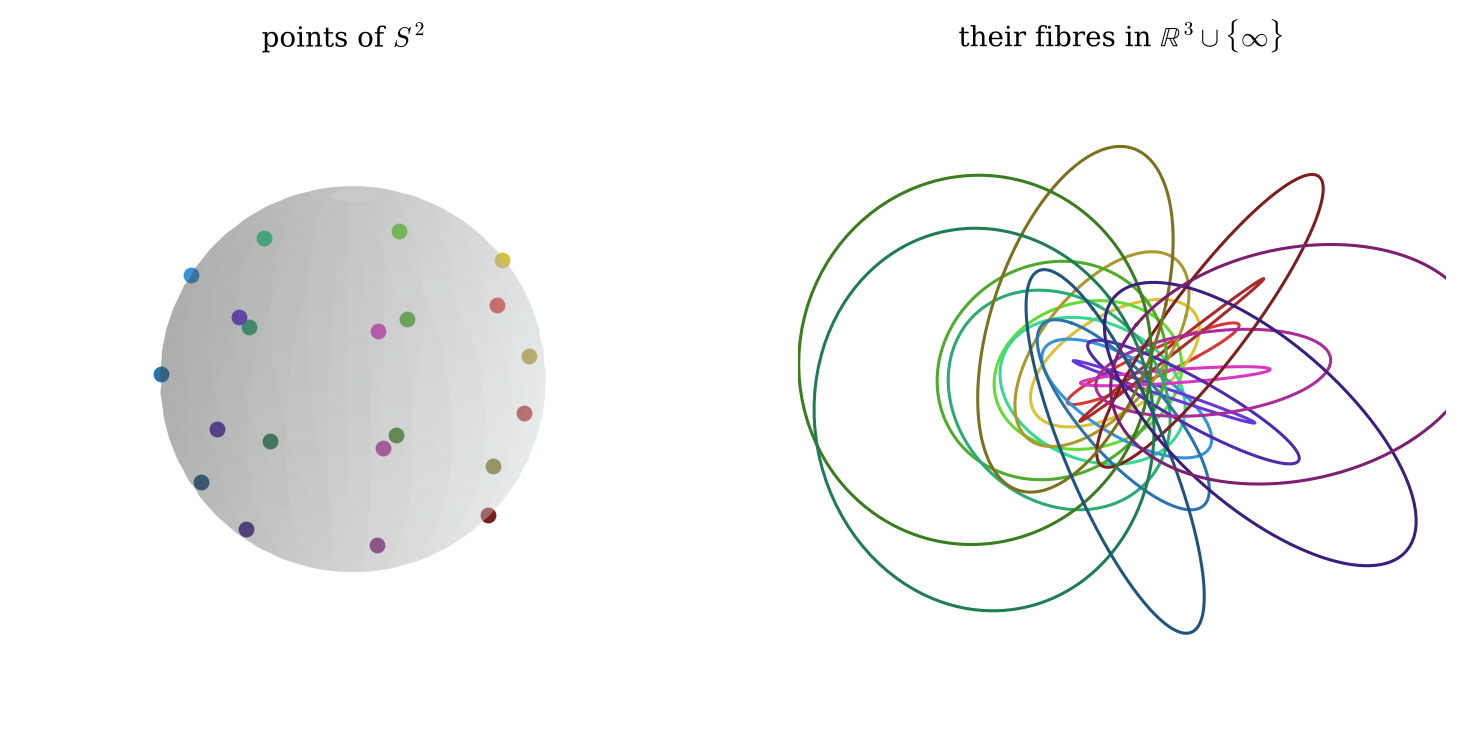
\includegraphics[width=0.92\textwidth]{fig_base_and_fibres.png}
\caption{Left: points on the base $S^2$. Right: the corresponding fibres of $h\colon S^3\to S^2$ after stereographic projection to $\R^3$, in the same colours. Points on one circle of latitude give fibres on one torus; the north pole gives the circle at infinity (here the vertical axis together with $\infty$), and the south pole gives the unit circle in the horizontal plane.}
\label{fig:basefibres}
\end{figure}

\subsection{The projective plane of the bundle}\label{sec:projplane}

For $d\ge2$ let $D(L_\K)$ be the unit disc bundle. It is a compact $2d$-manifold with boundary $S(L_\K)=S^{2d-1}$, and we put
\begin{equation}\label{eq:KP2}
\KP^2=D(L_\K)\cup_{S^{2d-1}}D^{2d},
\end{equation}
glued along the identity of $S^{2d-1}=\partial D^{2d}$. For $\K=\C,\Hq$ this is the complex or quaternionic projective plane, and for $\K=\Oc$ it is the Cayley plane;\footnote{We only use the topological description \eqref{eq:KP2}, which makes no reference to octonionic lines in $\Oc^3$.} we keep the notation $\KP^2$ in all three cases.

\begin{proposition}\label{prop:cone}
Let $d\in\{2,4,8\}$.
\begin{enumerate}[label=\textup{(\roman*)}]
\item $\KP^2$ is a closed, simply connected, hence orientable, topological $2d$-manifold.
\item $\KP^2$ is homeomorphic to the mapping cone $C_{h}=S^d\cup_{h_\K}D^{2d}$ of $h_\K$.
\item $H^j(\KP^2;\Z)\cong\Z$ for $j=0,d,2d$ and $H^j(\KP^2;\Z)=0$ otherwise.
\end{enumerate}
\end{proposition}

\begin{proof}
(ii) The disc bundle $D(L_\K)$ is homeomorphic to the mapping cylinder of the projection $S(L_\K)\to S^d$: the map $(v,t)\mapsto tv$ from $S(L_\K)\times[0,1]$ onto $D(L_\K)$ identifies exactly the points with $t=0$ in the same fibre. Gluing $D^{2d}$ to the mapping cylinder along its free end $S(L_\K)=S^{2d-1}$ gives the mapping cone.
(i) A manifold with boundary glued to another along a homeomorphism of their boundaries is a manifold, since boundaries have collar neighbourhoods. The space is compact and has no boundary. By (ii) it is a CW complex with one cell in each of the dimensions $0$, $d$ and $2d$; as $d\ge2$ there are no $1$-cells, so it is simply connected, and a simply connected manifold is orientable.
(iii) The cellular cochain complex has one generator in each of the degrees $0,d,2d$ and all differentials zero, because no two cells have adjacent dimensions.
\end{proof}
